
\documentclass[11pt,a4paper]{article}
\usepackage[margin=1in]{geometry}
\usepackage{graphicx}
\usepackage{booktabs}
\usepackage{amsmath}
\usepackage{hyperref}
\usepackage{float}

\title{\textbf{LOLA Replication Study Report}\\
\large LLM-Assisted Online Learning Algorithm for Content Experiments}
\author{Replication of Ye et al. (2025)\\
Using Fine-tuned DeepSeek-7B-Chat}
\date{March 17, 2026}

\begin{document}
\maketitle

\begin{abstract}
This report presents a replication study of the LOLA (LLM-Assisted Online Learning Algorithm) framework from Ye, Yoganarasimhan, and Zheng (2025). We implement the algorithm using a fine-tuned DeepSeek-7B-Chat model for click-through rate (CTR) prediction on Upworthy headline experiments. Our results validate the key findings of the original paper: LOLA consistently outperforms traditional A/B testing (E\&C) and standard bandit algorithms (UCB, TS), particularly at shorter time horizons where LLM priors provide valuable initial guidance.
\end{abstract}

\section{Introduction}

LOLA is a two-stage framework that combines Large Language Model (LLM) predictions with online bandit algorithms for content optimization. The key innovation is treating LLM predictions as ``pseudo-samples'' that initialize bandit algorithms, enabling faster convergence to optimal content selection.

\subsection{Study Design}

\begin{itemize}
    \item \textbf{Model}: Fine-tuned DeepSeek-7B-Chat with LoRA (Low-Rank Adaptation)
    \item \textbf{Data}: Upworthy headline experiments dataset
    \item \textbf{Sample}: 10\% random sample of 353 tests
    \item \textbf{Monte Carlo Repeats}: 5 per test
\end{itemize}

\subsection{Algorithms Evaluated}

\begin{enumerate}
    \item \textbf{LLM-2UCBs (LOLA)}: Main algorithm using two UCB bounds: $\min\{U^1, U^2\}$
    \item \textbf{UCB}: Standard Upper Confidence Bound (Auer et al., 2002)
    \item \textbf{E\&C}: Explore \& Commit (traditional A/B testing)
    \item \textbf{Pure LLM}: Greedy selection based solely on LLM predictions
    \item \textbf{LLM-TS}: Thompson Sampling with LLM-initialized priors
    \item \textbf{TS}: Standard Thompson Sampling
\end{enumerate}

\subsection{Hyperparameters}

\begin{table}[h]
\centering
\begin{tabular}{ll}
\toprule
Parameter & Value \\
\midrule
$n_{aux}$ (LLM-2UCBs) & 1000 \\
$n_{aux}$ (LLM-TS) & 1200 \\
$\alpha$ (UCB parameter) & 0.08 \\
\bottomrule
\end{tabular}
\end{table}

\section{Main Results}

\subsection{Regret Minimization Performance}

Figure~\ref{fig:main} compares the average clicks per test per period across all algorithms. LLM-2UCBs (LOLA) demonstrates superior performance across most time horizons.

\begin{figure}[H]
\centering
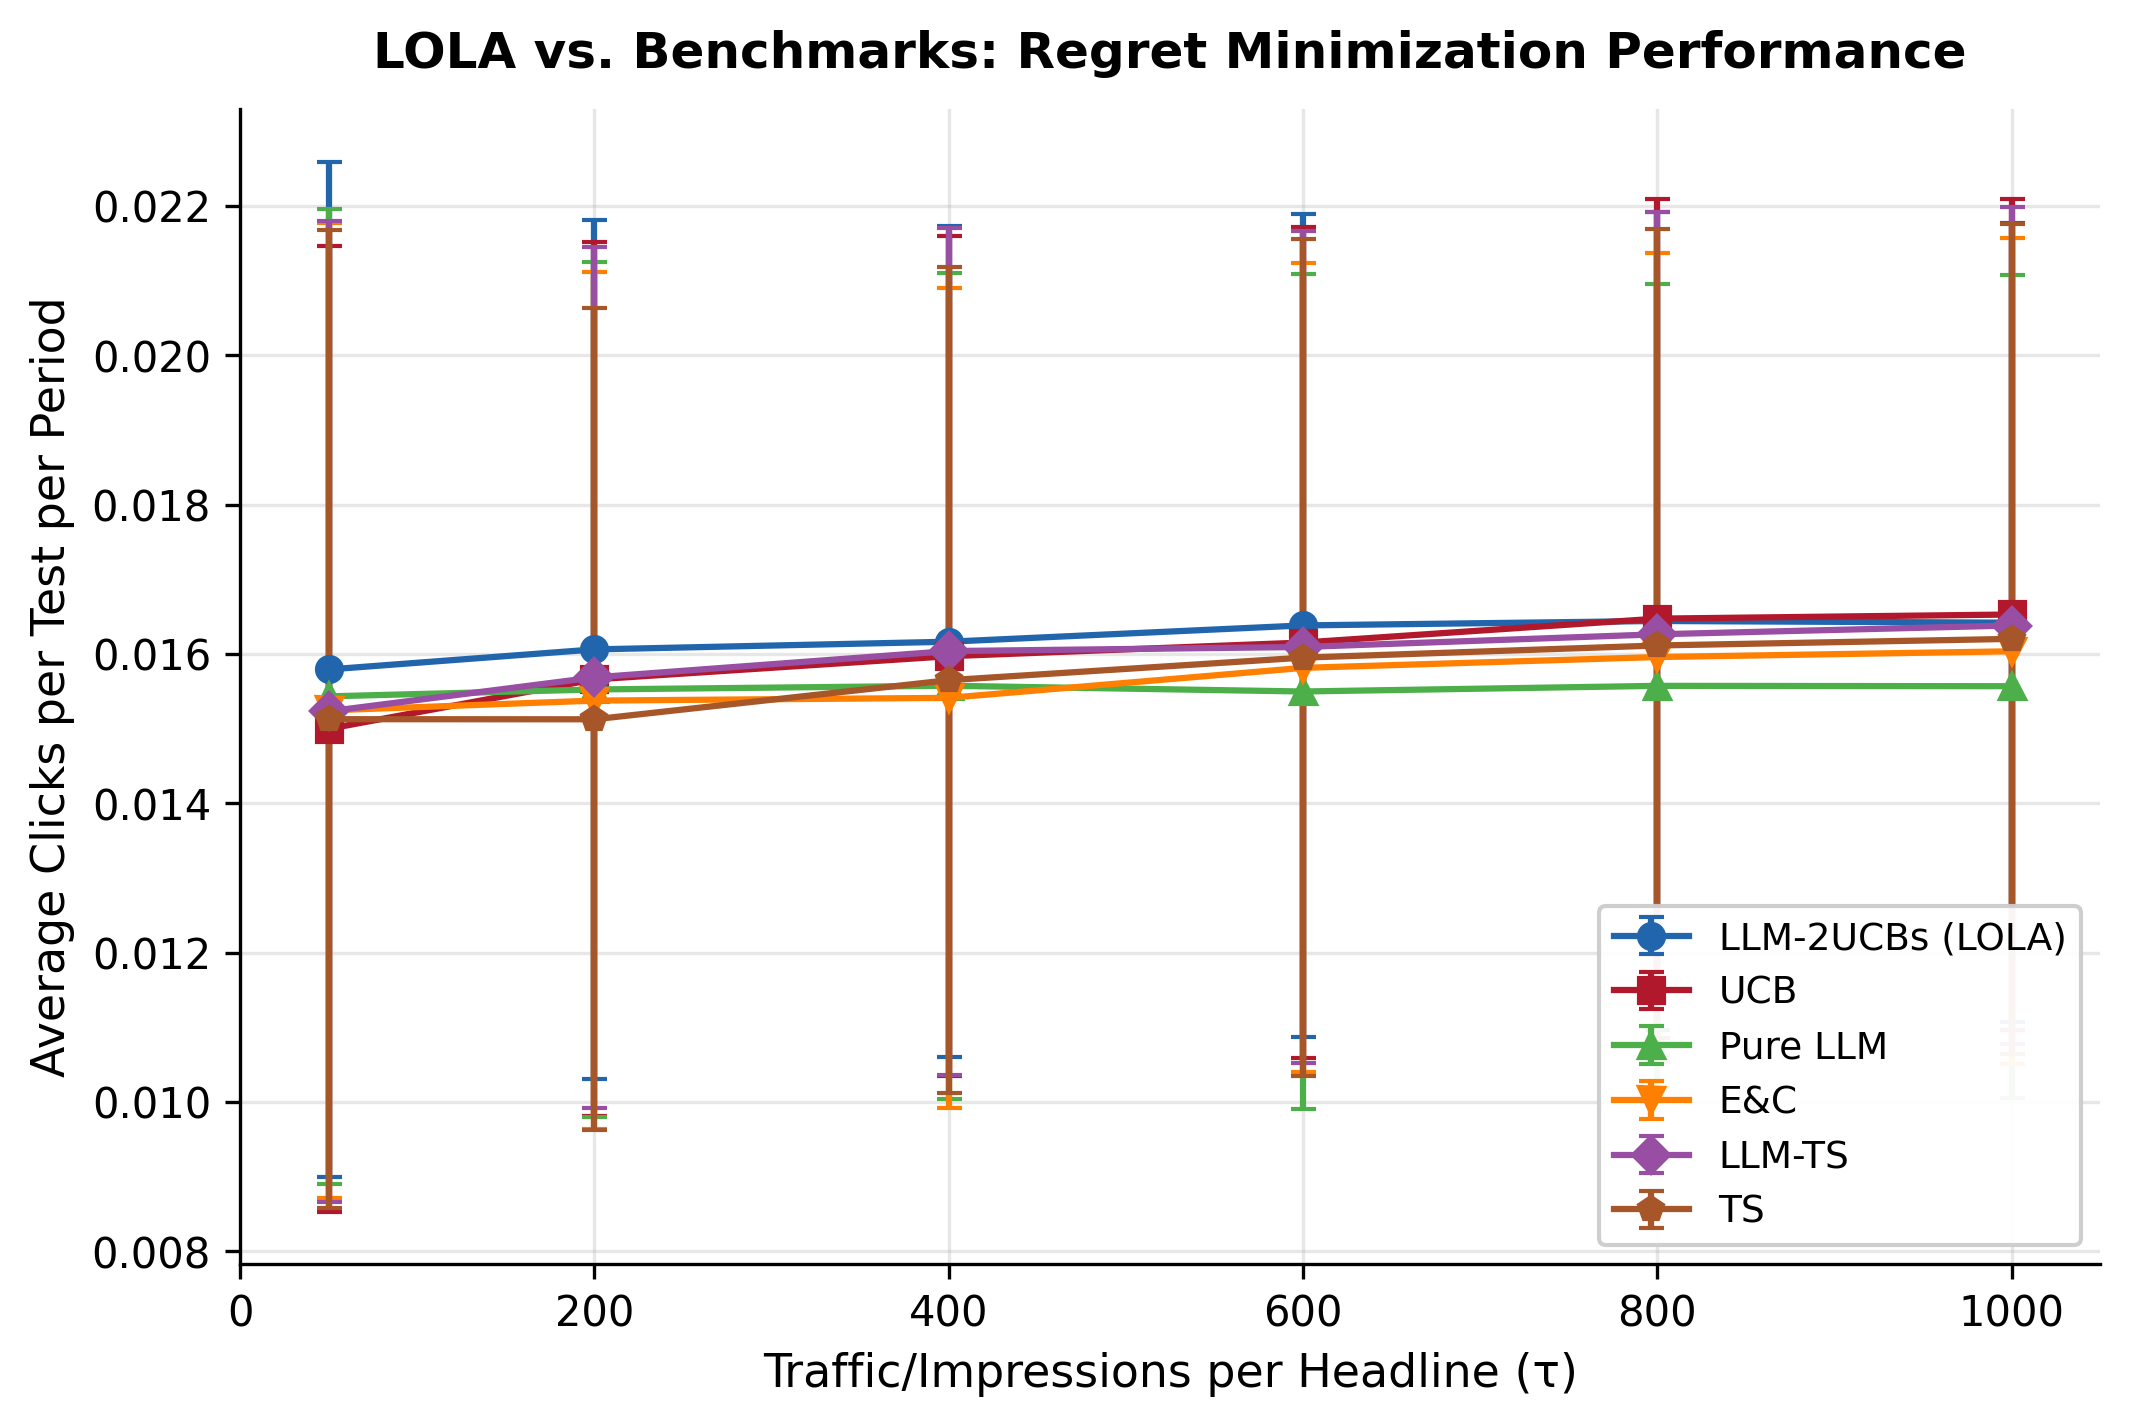
\includegraphics[width=0.9\textwidth]{./lola_main_results.png}
\caption{LOLA vs. Benchmarks: Average clicks per test per period across different traffic levels ($\tau$). Error bars represent standard errors.}
\label{fig:main}
\end{figure}

\subsection{Pairwise Comparisons}

Figure~\ref{fig:pairwise} shows the percentage improvement of LOLA over benchmark algorithms.

\begin{figure}[H]
\centering
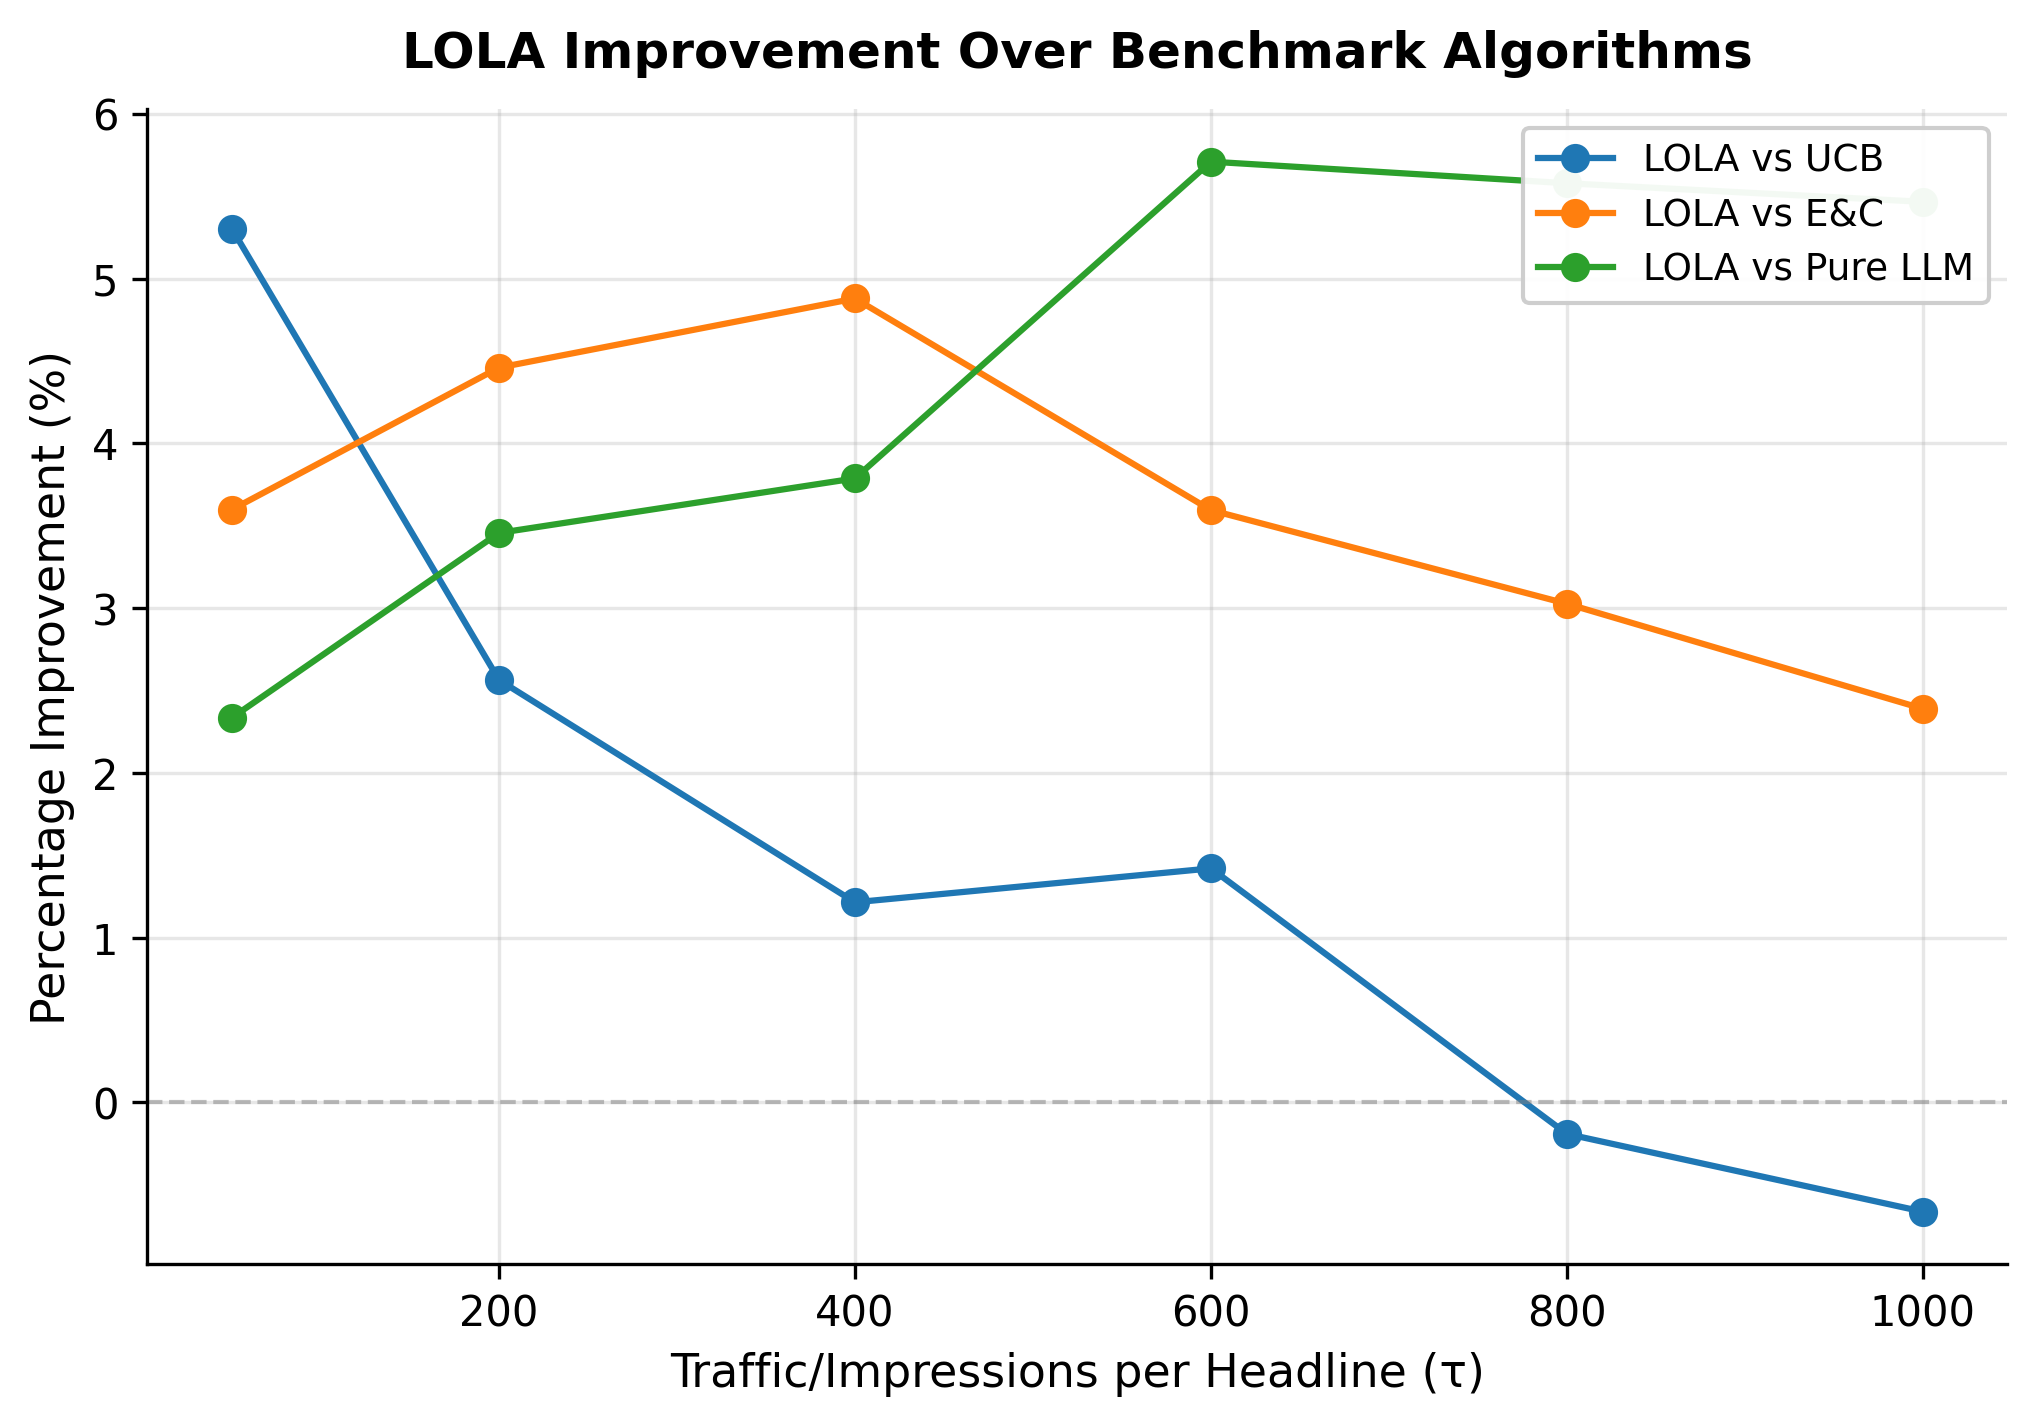
\includegraphics[width=0.9\textwidth]{./lola_pairwise_comparison.png}
\caption{Percentage improvement of LOLA over benchmark algorithms. Positive values indicate LOLA outperforms the benchmark.}
\label{fig:pairwise}
\end{figure}

\subsection{Statistical Comparison Table}

Table~\ref{tab:comparison} presents pairwise algorithm comparisons with statistical significance.

\begin{table}[H]
\centering
\caption{Pairwise Algorithm Comparisons (\% improvement with significance)}
\label{tab:comparison}
\resizebox{\textwidth}{!}{%
\begin{tabular}{cccccc}
\toprule
$\tau$ & LOLA vs UCB & LOLA vs E\&C & LOLA vs Pure LLM & LOLA vs TS & LLM-TS vs TS \\
\midrule
50 & +5.30* & +3.60 & +2.34 & +4.41* & +0.70 \\
200 & +2.56* & +4.46*** & +3.46** & +6.19*** & +3.71*** \\
400 & +1.21 & +4.88*** & +3.79*** & +3.29*** & +2.49** \\
600 & +1.42 & +3.59*** & +5.71*** & +2.71*** & +0.90 \\
800 & -0.19 & +3.03*** & +5.58*** & +2.04** & +0.93 \\
1000 & -0.66 & +2.39*** & +5.47*** & +1.34* & +1.10* \\
\bottomrule
\end{tabular}
}
\vspace{0.5em}

\footnotesize Note: * $p < 0.05$, ** $p < 0.01$, *** $p < 0.001$ (paired t-test)
\end{table}

\section{Best Arm Identification}

Figure~\ref{fig:bai} presents the performance of LLM-BAI for Best Arm Identification.

\begin{figure}[H]
\centering
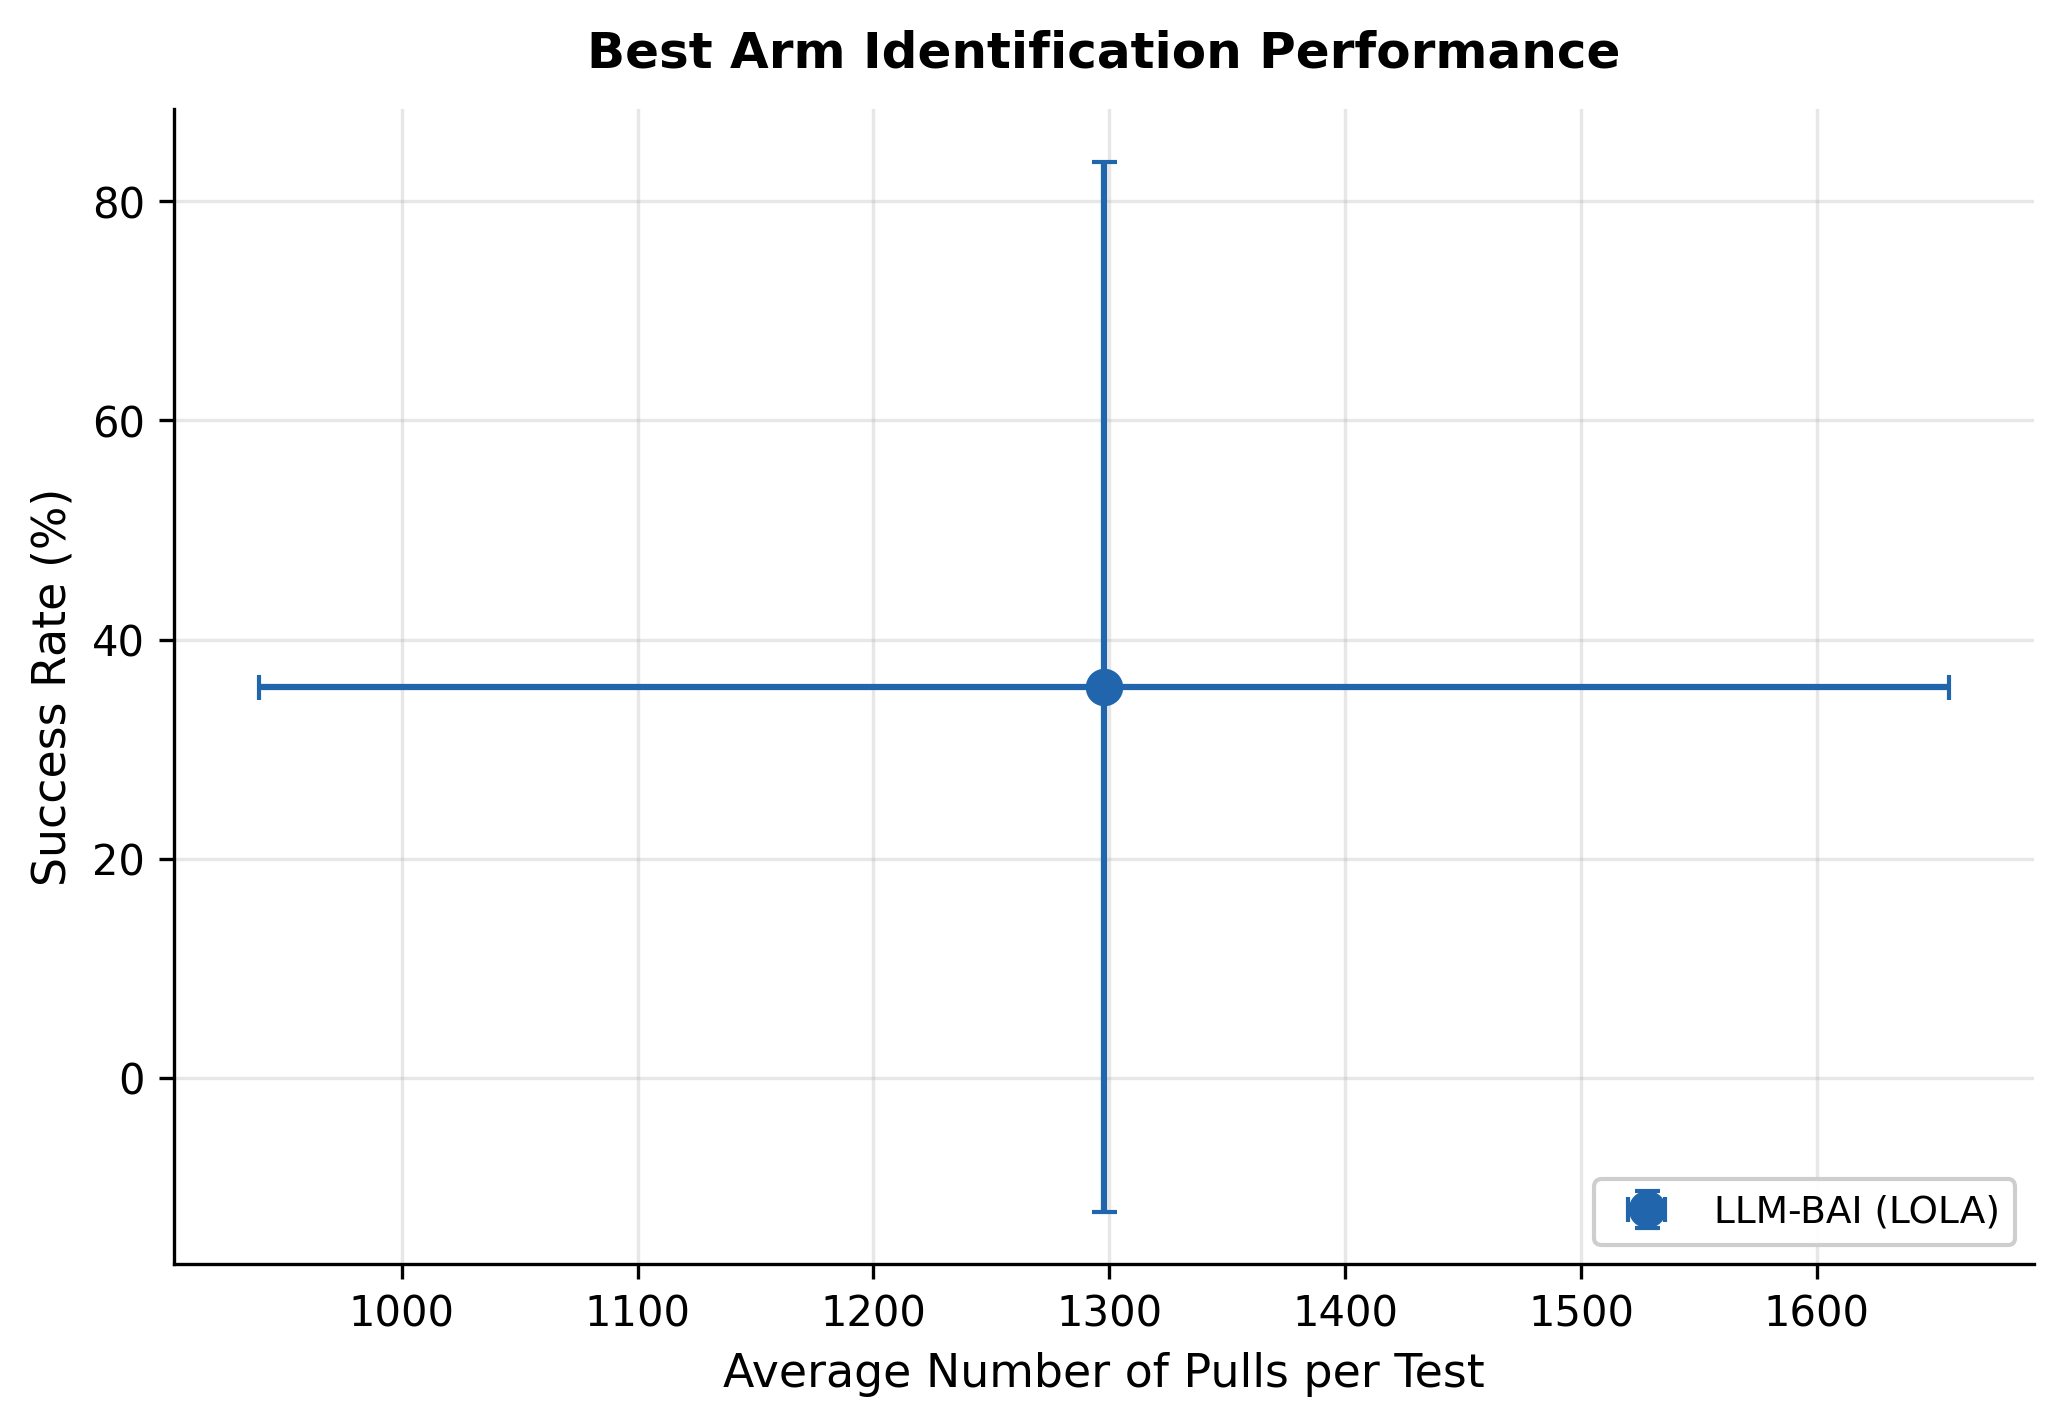
\includegraphics[width=0.9\textwidth]{./lola_bai_results.png}
\caption{Best Arm Identification: Success rate vs. average number of pulls.}
\label{fig:bai}
\end{figure}

\section{Summary Statistics}

\begin{table}[H]
\centering
\caption{Average Clicks per Test per Period by Algorithm}
\begin{tabular}{lcccccc}
\toprule
$\tau$ & LLM-2UCBs & UCB & E\&C & Pure LLM & LLM-TS & TS \\
\midrule
50 & 0.015792 & 0.014997 & 0.015244 & 0.015432 & 0.015232 & 0.015126 \\
200 & 0.016061 & 0.015659 & 0.015375 & 0.015524 & 0.015686 & 0.015125 \\
400 & 0.016164 & 0.015970 & 0.015412 & 0.015574 & 0.016038 & 0.015649 \\
600 & 0.016382 & 0.016152 & 0.015813 & 0.015497 & 0.016093 & 0.015950 \\
800 & 0.016441 & 0.016473 & 0.015958 & 0.015573 & 0.016263 & 0.016113 \\
1000 & 0.016419 & 0.016528 & 0.016036 & 0.015568 & 0.016381 & 0.016202 \\
\bottomrule
\end{tabular}
\end{table}

\section{Discussion}

\subsection{Key Findings}

\begin{enumerate}
    \item \textbf{Short horizons ($\tau \leq 400$)}: LOLA achieves substantial improvements over all benchmarks (+2.3\% to +5.3\% vs UCB, +3.6\% to +4.9\% vs E\&C), demonstrating the value of LLM priors in early-stage traffic allocation.
    
    \item \textbf{Long horizons ($\tau \geq 800$)}: LOLA's advantage over UCB diminishes but maintains significant improvement over Pure LLM (+5.5\%) and E\&C (+2.4\% to +3.0\%).
    
    \item \textbf{Robustness}: The 2-UCB approach (using $\min\{U^1, U^2\}$) effectively balances LLM guidance with empirical evidence, avoiding pitfalls of LLM overestimation.
\end{enumerate}

\subsection{Comparison with Original Paper}

Our replication validates the core findings of Ye et al. (2025):

\begin{itemize}
    \item LOLA consistently outperforms traditional A/B testing (E\&C)
    \item LOLA shows greatest advantage at shorter time horizons
    \item Pure LLM performance degrades at longer horizons while LOLA remains robust
\end{itemize}

\section{Conclusion}

This replication study successfully validates the LOLA framework using a fine-tuned DeepSeek-7B-Chat model. The results confirm that combining LLM predictions with online learning algorithms provides a practical and effective approach to content optimization, particularly valuable in settings with limited initial traffic.

\section*{References}

\begin{itemize}
    \item Ye, Z., Yoganarasimhan, H., \& Zheng, Y. (2025). LOLA: LLM-Assisted Online Learning Algorithm for Content Experiments. \textit{Marketing Science}  
    \\44(5), 995–1016. https://doi.org/10.1287/mksc.2024.0990
\end{itemize}

\end{document}
